% ============================================================
% 12-de-casteljau-plots-explained.tex
% Compile with:  pdflatex -shell-escape 12-de-casteljau-plots-explained.tex
% The PNG must be in the same folder. Run twice for TOC.
% ============================================================

\documentclass[12pt, a4paper]{article}

\usepackage[T1]{fontenc}
\usepackage[utf8]{inputenc}
\usepackage{lmodern}
\usepackage[top=2.5cm, bottom=2.5cm, left=2.8cm, right=2.8cm]{geometry}
\usepackage{graphicx}
\usepackage{float}
\usepackage[dvipsnames]{xcolor}

\definecolor{codebg}{RGB}{248,248,248}
\definecolor{rulecolor}{RGB}{180,180,180}
\definecolor{examplebg}{RGB}{240,248,255}
\definecolor{examplerule}{RGB}{100,149,237}
\definecolor{notebg}{RGB}{255,250,230}
\definecolor{noterule}{RGB}{210,180,50}

\usepackage{minted}
\setminted[julia]{
  bgcolor=codebg, frame=leftline, framerule=1.5pt,
  rulecolor=rulecolor, linenos=false, fontsize=\small,
  breaklines=true, tabsize=4, style=friendly,
}

\usepackage{amsmath}
\usepackage{amssymb}
\usepackage{tikz}
\usetikzlibrary{shapes.geometric, arrows.meta, positioning}
\usepackage{mdframed}

\newmdenv[backgroundcolor=examplebg, linecolor=examplerule,
  linewidth=1.5pt, leftline=true, rightline=false,
  topline=false, bottomline=false,
  innerleftmargin=10pt, innerrightmargin=8pt,
  innertopmargin=6pt, innerbottommargin=6pt,
  skipabove=6pt, skipbelow=4pt]{examplebox}

\newmdenv[backgroundcolor=notebg, linecolor=noterule,
  linewidth=1.5pt, leftline=true, rightline=false,
  topline=false, bottomline=false,
  innerleftmargin=10pt, innerrightmargin=8pt,
  innertopmargin=6pt, innerbottommargin=6pt,
  skipabove=6pt, skipbelow=4pt]{notebox}

\usepackage[colorlinks=true, linkcolor=black, urlcolor=MidnightBlue]{hyperref}
\usepackage{booktabs}
\usepackage{needspace}
\usepackage{parskip}
\usepackage{titlesec}
\usepackage{fancyhdr}
\usepackage{datetime2}

\titleformat{\section}
  {\large\bfseries\color{MidnightBlue}}{\thesection.}{0.6em}{}
  [\vspace{-4pt}\rule{\linewidth}{0.4pt}]
\titleformat{\subsection}
  {\normalsize\bfseries\color{BrickRed}}{\thesubsection.}{0.5em}{}
\titleformat{\subsubsection}
  {\normalsize\bfseries}{\thesubsubsection.}{0.5em}{}

\pagestyle{fancy}
\fancyhf{}
\rhead{\textcolor{gray}{\small 12-de-casteljau-plots-explained}}
\lhead{\textcolor{gray}{\small De Casteljau --- Plots.jl}}
\cfoot{\thepage}
\renewcommand{\headrulewidth}{0.3pt}

\newcommand{\cd}[1]{\texttt{#1}}

\title{%
  \vspace{1cm}
  {\LARGE\bfseries De Casteljau Algorithm}\\[0.4em]
  {\large Quadratic B\'ezier --- Plots.jl Visualisation}\\[0.4em]
  {\large Code and Plot Explanation for Julia Beginners}\\[0.4em]
  {\normalsize\texttt{12-de-casteljau-plots.jl}}
}
\author{E.R.\ Nurwijayadi}
\date{\DTMtoday}

\begin{document}

\maketitle
\thispagestyle{empty}

\begin{center}
\textit{Directed and curated by E.R.\ Nurwijayadi.
Code and explanations AI-generated.}
\end{center}

\begin{center}
\begin{minipage}{0.85\textwidth}
\small
This document explains \cd{12-de-casteljau-plots.jl}.
The script visualises the \textbf{De Casteljau algorithm}
--- a geometric method for evaluating B\'ezier curves ---
applied to the same quadratic curve as script~11.
New concepts: linear interpolation (\cd{lerp}), multi-level
geometric construction, named tuple return values, and
plotting multiple coloured snapshots of the algorithm.
\end{minipage}
\end{center}

\vspace{1em}\hrule\vspace{1.5em}
\tableofcontents
\newpage


% =============================================================
\needspace{8\baselineskip}
\section{The Plot}
% =============================================================

\begin{figure}[H]
  \centering
  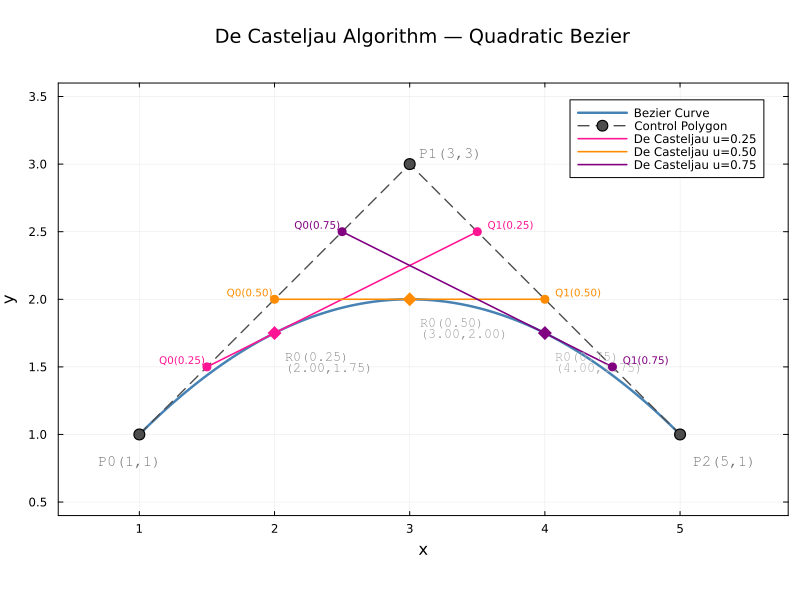
\includegraphics[width=0.95\linewidth]{12-bezier-decasteljau-plots.png}
  \caption{De Casteljau algorithm at $u=0.25$ (pink),
           $u=0.50$ (orange), $u=0.75$ (purple).}
  \label{fig:decasteljau}
\end{figure}


% =============================================================
\needspace{8\baselineskip}
\section{The De Casteljau Algorithm --- What Is It?}
% =============================================================

\textit{Script~11 evaluated the B\'ezier curve using the
Bernstein polynomial formula.
This script shows a completely different approach that
produces the exact same curve, but geometrically.}

The \textbf{De Casteljau algorithm} evaluates a B\'ezier
curve at parameter $u$ by repeated linear interpolation.
For a quadratic curve with control points $P_0$, $P_1$, $P_2$:

\textbf{Level 0 (given):} the three control points.

\textbf{Level 1 (interpolate):} compute two new points by
interpolating between adjacent control points at ratio $u$:
\[
  Q_0 = (1-u) P_0 + u P_1
  \qquad
  Q_1 = (1-u) P_1 + u P_2
\]

\textbf{Level 2 (interpolate again):} compute one final point
by interpolating between $Q_0$ and $Q_1$ at ratio $u$:
\[
  R_0 = (1-u) Q_0 + u Q_1
\]

$R_0$ is the point on the B\'ezier curve at parameter $u$.
Repeating this for all $u \in [0,1]$ traces the full curve.

\begin{notebox}
\textbf{Why is this useful?}
De Casteljau is numerically stable (no polynomial evaluation,
no large powers), easy to implement recursively for any degree,
and forms the basis of curve subdivision algorithms used in
font rendering and CAD software.
The Bernstein formula and De Casteljau always give the same
curve point --- they are two ways of computing the same thing.
\end{notebox}


% =============================================================
\needspace{8\baselineskip}
\section{Reading the Plot}
% =============================================================

\needspace{5\baselineskip}
\subsection{Background elements}

\textbf{Blue curve} --- the full B\'ezier curve, same as script~11.

\textbf{Gray dashed polygon with black dots} --- the control polygon
connecting $P_0(1,1)$, $P_1(3,3)$, $P_2(5,1)$.

\needspace{5\baselineskip}
\subsection{The three coloured snapshots}

The algorithm is shown at three values of $u$, each in a
different colour. For each snapshot:

\begin{itemize}
  \item A \textbf{solid coloured line} connects $Q_0$ and $Q_1$
        (the level-1 intermediate points).
        This line is the ``level-1 construction segment.''
  \item Two \textbf{small filled circles} mark $Q_0$ and $Q_1$
        with labels \cd{Q0(u)} and \cd{Q1(u)}.
  \item A \textbf{diamond} marks $R_0$ --- the final curve point
        at that $u$ value. The diamond sits exactly on the blue curve.
  \item A \textbf{label} below the diamond shows
        \cd{R0(u) / (x, y)}.
\end{itemize}

\begin{examplebox}
\textbf{Reading the $u = 0.50$ snapshot (orange):}

$Q_0(0.50)$ is the midpoint of $P_0P_1$:
$(1+3)/2 = 2,\; (1+3)/2 = 2$ $\to$ $(2, 2)$.

$Q_1(0.50)$ is the midpoint of $P_1P_2$:
$(3+5)/2 = 4,\; (3+1)/2 = 2$ $\to$ $(4, 2)$.

$R_0(0.50)$ is the midpoint of $Q_0Q_1$:
$(2+4)/2 = 3,\; (2+2)/2 = 2$ $\to$ $(3, 2)$.

This matches the orange diamond at $(3.00, 2.00)$
on the plot. \checkmark

The orange construction segment is the horizontal line
from $(2, 2)$ to $(4, 2)$.
\end{examplebox}

\begin{examplebox}
\textbf{Reading the $u = 0.25$ snapshot (pink):}

$Q_0(0.25) = 0.75 \cdot P_0 + 0.25 \cdot P_1
= 0.75(1,1) + 0.25(3,3) = (1.5, 1.5)$.

$Q_1(0.25) = 0.75 \cdot P_1 + 0.25 \cdot P_2
= 0.75(3,3) + 0.25(5,1) = (3.5, 2.5)$.

$R_0(0.25) = 0.75 \cdot Q_0 + 0.25 \cdot Q_1
= 0.75(1.5, 1.5) + 0.25(3.5, 2.5) = (2.0, 1.75)$.

The pink diamond sits at $(2.00, 1.75)$. \checkmark
\end{examplebox}

\needspace{5\baselineskip}
\subsection{What the construction lines reveal}

The coloured construction segments $Q_0Q_1$ visually show
how the curve point is ``found'' geometrically:
the curve point $R_0$ always lies on its construction
segment, at fraction $u$ along that segment.
The three crossing construction lines in the plot illustrate
why the algorithm is elegant --- each line narrows in on
the curve from a different angle.


% =============================================================
\needspace{8\baselineskip}
\section{Type Map}
% =============================================================

\tikzset{
  structbox/.style={rectangle, rounded corners=4pt,
    draw=MidnightBlue, line width=1.5pt, fill=examplebg,
    text width=3.4cm, align=center, font=\small\bfseries, inner sep=8pt},
  funcbox/.style={rectangle, rounded corners=2pt,
    draw=gray!60, line width=1pt, fill=white,
    text width=3.4cm, align=center, font=\small, inner sep=7pt},
  entrybox/.style={rectangle, rounded corners=4pt,
    draw=BrickRed, line width=1.5pt, fill=notebg,
    text width=2.4cm, align=center, font=\small\bfseries, inner sep=8pt},
  myarrow/.style={-Stealth, thick, draw=gray!70},
  bluearrow/.style={-Stealth, thick, draw=MidnightBlue},
  redarrow/.style={-Stealth, thick, draw=BrickRed!80},
  arrowlabel/.style={font=\footnotesize\itshape, fill=white, inner sep=2pt}
}

\begin{center}
\begin{tikzpicture}[node distance=1.5cm and 2.8cm]

  \node[structbox] (dc) {%
    \texttt{DeCasteljauQuadratic}\\[3pt]
    \footnotesize\normalfont
    \texttt{p0, p1, p2}\\
    \texttt{::Vector\{Float64\}}
  };

  \node[funcbox, below left=1.5cm and 0.2cm of dc] (math) {%
    \textbf{Math functions}\\[2pt]
    \footnotesize\normalfont
    \texttt{lerp(a, b, u)}\\
    \texttt{steps(dc, u)}\\
    \texttt{dc\_curve(dc, n)}
  };

  \node[funcbox, below right=1.5cm and 0.2cm of dc] (draw) {%
    \texttt{draw\_and\_save}\\[2pt]
    \footnotesize\normalfont
    \textit{curve + polygon layer}\\
    \textit{loop: 3 snapshots}\\
    \textit{each: segment, dots,}\\
    \textit{diamond, labels}
  };

  \node[entrybox, right=2.2cm of dc] (main) {%
    \texttt{main()}\\[2pt]
    \footnotesize\normalfont\normalcolor
    \textit{entry point}
  };

  \draw[bluearrow] (dc)   -- node[arrowlabel,above left]{passed to} (math);
  \draw[bluearrow] (dc)   -- node[arrowlabel,above right]{passed to} (draw);
  \draw[myarrow]   (draw) -- node[arrowlabel,below]{calls} (math);
  \draw[redarrow]  (main) -- node[arrowlabel,above]{creates} (dc);
  \draw[redarrow]  (main) |- node[arrowlabel,right,pos=0.8]{calls} (draw);

\end{tikzpicture}
\end{center}


% =============================================================
\needspace{8\baselineskip}
\section{Data and Constants}
% =============================================================

\begin{minted}{julia}
const CONTROL_POINTS = [
    1.0  1.0;   # P0
    3.0  3.0;   # P1
    5.0  1.0;   # P2
]

const U_SNAPSHOTS     = [0.25, 0.50, 0.75]
const SNAPSHOT_COLORS = [:deeppink, :darkorange, :purple]
\end{minted}

\cd{CONTROL\_POINTS} is identical to script~11.

\cd{U\_SNAPSHOTS} lists the three $u$ values at which the
De Casteljau construction is drawn.
\cd{SNAPSHOT\_COLORS} is a \cd{Vector\{Symbol\}} of
colour names --- one per snapshot.
The two vectors are paired: $u=0.25$ uses \cd{:deeppink},
$u=0.50$ uses \cd{:darkorange}, $u=0.75$ uses \cd{:purple}.

These pairs are iterated together with \cd{zip} in the
drawing loop, which is why the pink lines correspond to
$u=0.25$ and so on.


% =============================================================
\needspace{8\baselineskip}
\section{The \texttt{DeCasteljauQuadratic} Struct}
% =============================================================

\begin{minted}{julia}
struct DeCasteljauQuadratic
    p0::Vector{Float64}
    p1::Vector{Float64}
    p2::Vector{Float64}
end

DeCasteljauQuadratic(pts::Matrix{Float64}) =
    DeCasteljauQuadratic(pts[1,:], pts[2,:], pts[3,:])
\end{minted}

Identical in structure to \cd{BezierQuadratic} from
script~11 --- same three vector fields, same row-slice
constructor.
The name change from \cd{BezierQuadratic} to
\cd{DeCasteljauQuadratic} signals the different algorithm
used to evaluate it.


% =============================================================
\needspace{8\baselineskip}
\section{The Math Functions}
% =============================================================

\needspace{5\baselineskip}
\subsection{\texttt{lerp} --- linear interpolation}

\begin{minted}{julia}
lerp(a, b, u) = (1 - u) .* a .+ u .* b
\end{minted}

\cd{lerp} stands for \textbf{linear interpolation}.
Given two points \cd{a} and \cd{b} and a parameter
\cd{u} $\in [0, 1]$, it returns the point that is fraction
$u$ of the way from \cd{a} to \cd{b}:
\[
  \text{lerp}(a, b, u) = (1-u)\,a + u\,b
\]

At $u=0$ the result is exactly \cd{a}.
At $u=1$ the result is exactly \cd{b}.
At $u=0.5$ the result is the midpoint.

The broadcast operators \cd{.*} and \cd{.+} make this work
for both scalar arguments and 2-D point vectors without
any change to the formula.

\begin{examplebox}
\textbf{Scalar lerp:} \cd{lerp(1.0, 5.0, 0.25)}
$= 0.75 \times 1.0 + 0.25 \times 5.0 = 2.0$

\textbf{Vector lerp:}
\cd{lerp([1.0, 1.0], [3.0, 3.0], 0.25)}
$= 0.75 \times [1,1] + 0.25 \times [3,3]$
$= [0.75, 0.75] + [0.75, 0.75]$
$= [1.5, 1.5]$

This is $Q_0$ at $u=0.25$ --- the point $\tfrac{1}{4}$ of the
way from $P_0$ to $P_1$.
\end{examplebox}

\needspace{5\baselineskip}
\subsection{\texttt{steps} --- one full De Casteljau construction}

\begin{minted}{julia}
function steps(dc::DeCasteljauQuadratic, u::Float64)
    q0 = lerp(dc.p0, dc.p1, u)
    q1 = lerp(dc.p1, dc.p2, u)
    r0 = lerp(q0, q1, u)
    return (
        level0 = vcat(dc.p0', dc.p1', dc.p2'),
        level1 = vcat(q0',    q1'),
        level2 = r0,
    )
end
\end{minted}

\textbf{The computation:}
Three \cd{lerp} calls implement the two levels of
De Casteljau interpolation.
\cd{q0} and \cd{q1} are the level-1 points;
\cd{r0} is the final curve point.

\textbf{Named tuple return:}
The function returns a \textbf{named tuple} ---
a tuple where each element has a name.
In Julia, \cd{(level0 = ..., level1 = ..., level2 = ...)}
creates a named tuple.
The caller accesses fields by name:
\cd{s.level0}, \cd{s.level1}, \cd{s.level2}.

This is more readable than returning a plain tuple
\cd{(matrix1, matrix2, vector)} and having to remember
which position is which.

\textbf{The data in each level:}

\cd{level0} is the $3 \times 2$ control point matrix
(same shape as \cd{cp} in script~11).
Built by stacking three transposed row vectors with \cd{vcat}.

\cd{level1} is a $2 \times 2$ matrix holding $Q_0$ and
$Q_1$ as rows.
Built by stacking two transposed row vectors.

\cd{level2} is a length-2 vector holding $R_0 = (x, y)$.

\begin{examplebox}
\textbf{Full \cd{steps(dc, 0.25)} output:}

\[
  \text{\cd{level0}} =
  \begin{bmatrix} 1.0 & 1.0 \\ 3.0 & 3.0 \\ 5.0 & 1.0 \end{bmatrix}
  \quad \text{(always the same --- control points)}
\]

$Q_0 = \text{lerp}(P_0, P_1, 0.25) = (1.5, 1.5)$

$Q_1 = \text{lerp}(P_1, P_2, 0.25) = (3.5, 2.5)$

\[
  \text{\cd{level1}} =
  \begin{bmatrix} 1.5 & 1.5 \\ 3.5 & 2.5 \end{bmatrix}
\]

$R_0 = \text{lerp}(Q_0, Q_1, 0.25) = (2.0, 1.75)$

\[
  \text{\cd{level2}} = [2.0,\ 1.75]
\]
\end{examplebox}

\begin{examplebox}
\textbf{Full \cd{steps(dc, 0.50)} output:}

$Q_0 = \text{lerp}(P_0, P_1, 0.50) = (2.0, 2.0)$

$Q_1 = \text{lerp}(P_1, P_2, 0.50) = (4.0, 2.0)$

\[
  \text{\cd{level1}} =
  \begin{bmatrix} 2.0 & 2.0 \\ 4.0 & 2.0 \end{bmatrix}
\]

$R_0 = \text{lerp}(Q_0, Q_1, 0.50) = (3.0, 2.0)$

\[
  \text{\cd{level2}} = [3.0,\ 2.0]
\]

This explains the flat orange construction segment
(both $Q$ points have $y=2$) and the diamond exactly at
the peak of the curve.
\end{examplebox}

\begin{examplebox}
\textbf{Full \cd{steps(dc, 0.75)} output:}

$Q_0 = \text{lerp}(P_0, P_1, 0.75) = (2.5, 2.5)$

$Q_1 = \text{lerp}(P_1, P_2, 0.75) = (4.5, 1.5)$

\[
  \text{\cd{level1}} =
  \begin{bmatrix} 2.5 & 2.5 \\ 4.5 & 1.5 \end{bmatrix}
\]

$R_0 = \text{lerp}(Q_0, Q_1, 0.75) = (4.0, 1.75)$

\[
  \text{\cd{level2}} = [4.0,\ 1.75]
\]
\end{examplebox}

\needspace{5\baselineskip}
\subsection{\texttt{dc\_curve} --- the full curve via De Casteljau}

\begin{minted}{julia}
function dc_curve(dc::DeCasteljauQuadratic, n::Int=200)
    u_vals = LinRange(0.0, 1.0, n)
    hcat([steps(dc, u).level2 for u in u_vals]...)'
end
\end{minted}

For each of 200 $u$ values, calls \cd{steps(dc, u)} and
extracts only \cd{.level2} --- the final curve point.
The \cd{.level2} after the function call is
\textbf{field access on the return value}:
it reads the \cd{level2} field of the named tuple
returned by \cd{steps}, without storing the tuple in
a variable first.

The rest of the function (\cd{hcat}, splat, transpose)
is identical to \cd{curve()} in script~11 ---
same pattern, same result shape ($200 \times 2$).

\begin{examplebox}
\textbf{Content of \cd{cpts = dc\_curve(dc)} (first and last few rows):}

\medskip
\begin{center}
\begin{tabular}{rcc}
\toprule
Row & $x$ & $y$ \\
\midrule
1   & 1.0000 & 1.0000 \\
2   & 1.0402 & 1.0793 \\
$\vdots$ & $\vdots$ & $\vdots$ \\
100 & 3.0000 & 2.0000 \\
$\vdots$ & $\vdots$ & $\vdots$ \\
200 & 5.0000 & 1.0000 \\
\bottomrule
\end{tabular}
\end{center}

This is the same curve as script~11 --- the De Casteljau
algorithm and Bernstein formula always produce the same
curve points. Only the computation path differs.
\end{examplebox}


% =============================================================
\needspace{8\baselineskip}
\section{\texttt{draw\_and\_save} --- Building the Plot}
% =============================================================

\needspace{5\baselineskip}
\subsection{Base figure and static layers}

The \cd{plot()} call, the curve layer (\cd{plot!(plt, cpts...)}),
and the control polygon layer are identical in structure
to script~11.
One difference: the control polygon here uses
\cd{COLOR\_POLYGON = :gray30} (dark grey) instead of
crimson, giving the background skeleton a more neutral look
so the coloured snapshots stand out.

The control polygon is extracted via \cd{steps(dc, 0.0).level0}
rather than constructing it with \cd{vcat(bz.p0', bz.p1', bz.p2')}
directly.
At $u=0$, \cd{level0} always returns the full control
point matrix --- calling \cd{steps} is consistent with
the rest of the code even if slightly roundabout.

\needspace{5\baselineskip}
\subsection{The snapshot loop}

\begin{minted}{julia}
for (u, color) in zip(u_snapshots, colors)
    s  = steps(dc, u)
    l1 = s.level1
    r0 = s.level2
    ...
end
\end{minted}

\cd{zip(u\_snapshots, colors)} pairs each $u$ value with
its colour: \cd{(0.25, :deeppink)}, \cd{(0.50, :darkorange)},
\cd{(0.75, :purple)}.
Each iteration draws one full De Casteljau snapshot.

\cd{s = steps(dc, u)} calls the construction function once
and stores the full result.
\cd{l1 = s.level1} and \cd{r0 = s.level2} extract the
two fields needed for plotting.

\needspace{5\baselineskip}
\subsection{Level-1 segment and dots}

\begin{minted}{julia}
# Level-1 Q0-Q1 segment
plot!(plt, l1[:,1], l1[:,2],
    color     = color,
    linewidth = 1.6,
    label     = @sprintf("De Casteljau u=%.2f", u),
)

# Level-1 Q0, Q1 dots
scatter!(plt, l1[:,1], l1[:,2],
    color             = color,
    markersize        = 5,
    markerstrokewidth = 0,
    label             = false,
)
\end{minted}

\cd{l1[:,1]} and \cd{l1[:,2]} extract the $x$ and $y$
columns from the $2 \times 2$ level-1 matrix.
\cd{plot!} draws the construction segment; \cd{scatter!}
draws the two $Q$ dots on top of it.

\textbf{\cd{label = false}:}
The \cd{scatter!} call should not add a legend entry ---
the segment \cd{plot!} already provides the legend entry
for this snapshot.
Passing \cd{label = false} suppresses the legend entry
for that layer entirely.

\needspace{5\baselineskip}
\subsection{The level-2 diamond}

\begin{minted}{julia}
scatter!(plt,
    [r0[1]], [r0[2]],
    color             = color,
    marker            = :diamond,
    markersize        = 7,
    markerstrokewidth = 0,
    label             = false,
)
\end{minted}

\cd{r0} is a length-2 vector \cd{[x, y]}.
\cd{scatter!} expects vectors of coordinates, not scalar
values.
\cd{[r0[1]]} wraps the scalar $x$ value in a
length-1 vector; \cd{[r0[2]]} does the same for $y$.
This is necessary because \cd{scatter!(plt, x, y)}
requires both \cd{x} and \cd{y} to be arrays.

\cd{marker = :diamond} selects the diamond shape ---
the rotated square visible on the plot at each $R_0$ point.

\begin{examplebox}
\textbf{Why \cd{[r0[1]]} and not just \cd{r0[1]}?}

\cd{r0[1] = 2.0} (a scalar Float64).
Passing a scalar to \cd{scatter!} would cause a method
error.
\cd{[2.0]} is a length-1 vector \cd{Vector\{Float64\}},
which \cd{scatter!} accepts.

This pattern \cd{[scalar]} --- wrapping a single value
in square brackets to make it a vector --- is common in
Julia plotting code whenever you need to plot a single
isolated point.
\end{examplebox}

\needspace{5\baselineskip}
\subsection{Snapshot labels}

\begin{minted}{julia}
# Q0, Q1 labels
for (j, (qname, (dx, dy))) in enumerate(zip(["Q0","Q1"], Q_OFFSETS))
    annotate!(plt, l1[j,1]+dx, l1[j,2]+dy,
        text(@sprintf("%s(%.2f)", qname, u), color, :left, 7))
end

# R0 label
annotate!(plt, r0[1]+0.08, r0[2]-0.22,
    text(@sprintf("R0(%.2f)\n(%.2f,%.2f)", u, r0[1], r0[2]),
         color, :left, 7, :bold))
\end{minted}

The $Q$ label loop uses \cd{enumerate(zip(...))} to get
both the index \cd{j} (for accessing \cd{l1[j,1]}) and
the name/offset pair.
\cd{Q\_OFFSETS = [(-0.35, 0.05), (0.08, 0.05)]}
shifts $Q_0$ labels to the left (so they don't overlap
the construction line) and $Q_1$ labels to the right.

The \cd{R0} label includes both the $u$ value and the
$(x, y)$ coordinates, formatted in bold with a line break.

\begin{examplebox}
\textbf{All labels produced by the loop for $u = 0.25$ (pink):}

\medskip
\begin{tabular}{lll}
\toprule
Label & Text string & Position \\
\midrule
$Q_0$ & \cd{"Q0(0.25)"} & $(1.5-0.35,\; 1.5+0.05) = (1.15, 1.55)$ \\
$Q_1$ & \cd{"Q1(0.25)"} & $(3.5+0.08,\; 2.5+0.05) = (3.58, 2.55)$ \\
$R_0$ & \cd{"R0(0.25)\textbackslash n(2.00,1.75)"} & $(2.0+0.08,\; 1.75-0.22) = (2.08, 1.53)$ \\
\bottomrule
\end{tabular}
\end{examplebox}


% =============================================================
\needspace{8\baselineskip}
\section{Entry Point}
% =============================================================

\begin{minted}{julia}
function main()
    dc = DeCasteljauQuadratic(CONTROL_POINTS)
    draw_and_save(dc, U_SNAPSHOTS, SNAPSHOT_COLORS,
                  "12-bezier-decasteljau-plots.png")
end

main()
\end{minted}

\cd{draw\_and\_save} now takes four arguments instead of
three --- the snapshot $u$ values and colours are passed
in rather than being hardcoded inside the function.
This makes it easy to change the snapshots or colours
without editing the drawing function itself.

\begin{notebox}
\textbf{How to run:}
\begin{minted}{julia}
julia 12-de-casteljau-plots.jl
\end{minted}
Saves \cd{12-bezier-decasteljau-plots.png} and opens a window.
Press Enter to close.
\end{notebox}

\vspace{2em}\hrule\vspace{0.5em}
{\small\textcolor{gray}{%
Explanation for \texttt{12-de-casteljau-plots.jl}
\textbar{} Directed and curated by E.R.\ Nurwijayadi
\textbar{} Code and explanations AI-generated}}

\end{document}
